\documentclass[11pt]{article}

\usepackage{CMPSC465}
\usepackage{enumitem}
\usepackage{algpseudocode}
\usepackage{tikz}

\def\title{Assignment 03}

\def\defeq{\mathrel{\mathop:}=}
%\usepackage{algpseudocode}
%\usepackage{algorithm}
\usepackage[ruled,noline]{algorithm2e}
%\usepackage{amsthm}
\newcommand\nonl{%
  \renewcommand{\nl}{\let\nl\oldnl}}% Remove line number for one line
  
\newcommand{\aaa}[1]{\hspace{0.65cm}\parbox[t]{15.3cm}{#1}}
\newcommand{\aab}[1]{\hspace{1.15cm}\parbox[t]{15.0cm}{#1}}
\newcommand{\aac}[1]{\hspace{1.65cm}\parbox[t]{15.0cm}{#1}}
\newcommand{\aad}[1]{\hspace{2.15cm}\parbox[t]{15.0cm}{#1}}
\newcommand{\aaA}[2]{\hspace{0.5cm} {\tikz[overlay] \draw (0.1, -0.1) -- (0.1, #1 * -1.5em + 0.6em);} \parbox[t]{15.0cm}{#2}}
\newcommand{\aaB}[2]{\hspace{1.0cm} {\tikz[overlay] \draw (0.1, -0.1) -- (0.1, #1 * -1.5em + 0.6em);} \parbox[t]{15.0cm}{#2}}
\newcommand{\aaC}[2]{\hspace{1.5cm} {\tikz[overlay] \draw (0.1, -0.1) -- (0.1, #1 * -1.5em + 0.6em);} \parbox[t]{15.0cm}{#2}}
\newcommand{\aaD}[2]{\hspace{2.0cm} {\tikz[overlay] \draw (0.1, -0.1) -- (0.1, #1 * -1.5em + 0.6em);} \parbox[t]{15.0cm}{#2}}
\newcommand{\xxx}{\par\vspace{0.1cm}}

\begin{document}
\maketitle

\section*{Due: Friday 11:59 am, Feb.\ 04, 2022}

\paragraph*{Instructions:}

You may work in groups of up to three people to solve the homework.
You must write your own solutions and explicitly acknowledge everyone whom 
you have worked with or who has given you any significant ideas about your solutions. 
You may also use books or online resources to help solve homework problems.  
All consulted references must be acknowledged. The acknowledgements need to be made by answering Problem~1 below.

You are encouraged to solve the problem sets on your own using only the textbook and lecture notes as a reference. This will give you the best chance of doing well on the exams. Relying too much on the help of group members or on online resources will hinder your performance on the exams.

Submissions being late in 2 hours will be accepted with a 20\% penalty. Submissions late more than 2 hours will receive 0. There will be no exceptions to this policy, as we post the solutions soon after the deadline. 

For the full policy on assignments, please consult the syllabus.

\paragraph*{Formatting:} Start a new page for each problem.

\paragraph*{Describing an Algorithm:} Please make sure you use plain wording to explain your algorithm. It is always a good practice to start with a summary of the high-level idea of your algorithm to ease graders understand your solution quickly. Then, explain your algorithm, using plain wording and including enough details.

The use of pseudo-code is optional, and it is your decision. No matter you use it or not, above description in words is always required. The pseudo-code has its own advantage in explaining structured (i.e., if-else, for-loop, recursive functions, etc) algorithms and in putting details in the right place. If you think pseudo-code better explains your algorithm, and/or helps graders understand your solution, and/or contains more details not included in the plain-wording description, then use pseudo-code. If you think everything is already clearly explained in the description with words, then you don't need to include pseudo-code. An algorithm that is only written in pseudo-code (i.e., missing above plain-wording description) is not acceptable, as it is extremely hard to read just pseudo-code without any explanation.

Here is a general situation that may help you decide whether to use pseudo-code or not. An algorithm could be ``designed from scratch'', i.e., you will need to come up with the step-by-step procedure. This usually involves in implementing a function with clear input and output. In this case, including pseudo-code usually helps. All algorithm we've seen so far (e.g., merge-two-sorted-arrays, merge-sort, etc) falls in this category. Second, an algorithm could also be ''transformed into another algorithm'', i.e., you use an existing algorithm to solve this problem. In this case you usually don't need to include pseudo-code but to describe how to transform one problem into the other. We will see such examples soon.

\clearpage\newpage

\begin{qunlist}
\setcounter{sparectr}{-1}

\q{0}{Acknowledgements. }
	The assignment will receive a 0 if this question is not answered.
\begin{enumerate}
	\item If you worked in a group, list the members of the group. Otherwise, write ``I did not work in a group.''
	\item If you received significant ideas about your solutions from anyone not in your group, list their names here. Otherwise, write ``I did not consult  anyone except my group members''.
	\item List any resources besides the course material that you consulted in order to solve the material. If you did not consult anything, write ``I did not consult any non-class materials.''
\end{enumerate}

% from solution2.tex
\q{15}{}
Run the combine step of the divide-and-conquer algorithm for convex hull
on the instance given below. You are given $C_1 = (p_1, p_{10}, p_9, p_3, p_5)$
and $C_2 = (p_8, p_{6}, p_4, p_2, p_7, p_{11})$.
\begin{enumerate}
\item Find the lowest point $p^*$ in $C_1\cup C_2$.
\item Transform $C_1$ into $C_1'$ so that points in $C_1'$ is sorted in increasing angle w.r.t.\ $p^*$.
\item Partition $C_2$ into two lists $C_{2a}$ and $C_{2b}$ so that each list is sorted in increasing angle w.r.t.\ $p^*$.
\item Give list $C_2'$ by merging $C_{2a}$ and $C_{2b}$ so that each points in $C_2'$ is sorted in increasing angle w.r.t.\ $p^*$.
\item Give list $C'$ by merging $C_1'$ and $C_2'$ so that each points in $C'$ is sorted in increasing angle w.r.t.\ $p^*$.
\item Run Graham-Scan-Core algorithm to find convex hull of $C'$.
Show stack operations at each step (to deal with each point). For example,
you need to write like "For $A$: push $A$; pop $B$", which indicates when
you process point $A$, push $A$ into stack and also pop $B$ out.
\end{enumerate}

\begin{figure}[h]
\tikzset{every picture/.style={line width=0.75pt}} %set default line width to 0.75pt        

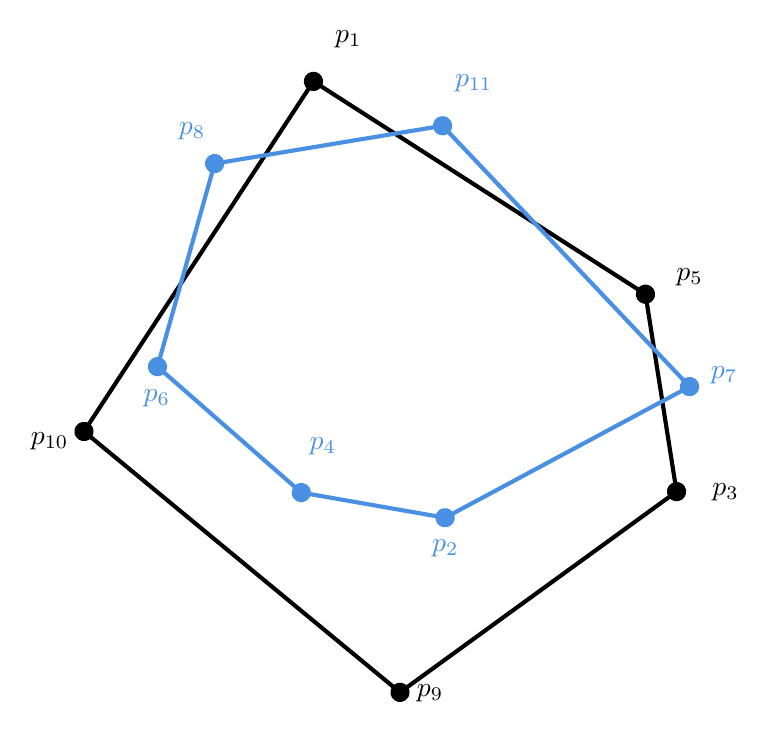
\begin{tikzpicture}[x=0.75pt,y=0.75pt,yscale=-1,xscale=1]
%uncomment if require: \path (0,391); %set diagram left start at 0, and has height of 391

%Flowchart: Connector [id:dp5289449572498183] 
\draw  [fill={rgb, 255:red, 0; green, 0; blue, 0 }  ,fill opacity=1 ] (239.33,364.26) .. controls (236.96,364.71) and (234.66,363.15) .. (234.21,360.78) .. controls (233.76,358.41) and (235.31,356.11) .. (237.69,355.66) .. controls (240.06,355.21) and (242.35,356.76) .. (242.81,359.14) .. controls (243.26,361.51) and (241.7,363.8) .. (239.33,364.26) -- cycle ;
%Flowchart: Connector [id:dp8854127292994846] 
\draw  [fill={rgb, 255:red, 0; green, 0; blue, 0 }  ,fill opacity=1 ] (87.06,238.59) .. controls (84.68,239.04) and (82.39,237.48) .. (81.94,235.11) .. controls (81.49,232.73) and (83.04,230.44) .. (85.42,229.99) .. controls (87.79,229.54) and (90.08,231.09) .. (90.54,233.47) .. controls (90.99,235.84) and (89.43,238.13) .. (87.06,238.59) -- cycle ;
%Flowchart: Connector [id:dp8118075796329792] 
\draw  [fill={rgb, 255:red, 0; green, 0; blue, 0 }  ,fill opacity=1 ] (357.58,172.44) .. controls (355.2,172.89) and (352.91,171.33) .. (352.46,168.96) .. controls (352,166.58) and (353.56,164.29) .. (355.94,163.84) .. controls (358.31,163.39) and (360.6,164.94) .. (361.05,167.32) .. controls (361.51,169.69) and (359.95,171.98) .. (357.58,172.44) -- cycle ;
%Flowchart: Connector [id:dp9423872091684253] 
\draw  [fill={rgb, 255:red, 0; green, 0; blue, 0 }  ,fill opacity=1 ] (372.56,267.55) .. controls (370.18,268.01) and (367.89,266.45) .. (367.44,264.08) .. controls (366.98,261.7) and (368.54,259.41) .. (370.92,258.96) .. controls (373.29,258.5) and (375.58,260.06) .. (376.04,262.43) .. controls (376.49,264.81) and (374.93,267.1) .. (372.56,267.55) -- cycle ;
%Flowchart: Connector [id:dp4355711900011987] 
\draw  [color={rgb, 255:red, 74; green, 144; blue, 226 }  ,draw opacity=1 ][fill={rgb, 255:red, 74; green, 144; blue, 226 }  ,fill opacity=1 ] (261.03,280.14) .. controls (258.66,280.59) and (256.37,279.04) .. (255.91,276.66) .. controls (255.46,274.29) and (257.02,272) .. (259.39,271.54) .. controls (261.77,271.09) and (264.06,272.65) .. (264.51,275.02) .. controls (264.96,277.39) and (263.41,279.69) .. (261.03,280.14) -- cycle ;
%Flowchart: Connector [id:dp42853879075832446] 
\draw  [fill={rgb, 255:red, 0; green, 0; blue, 0 }  ,fill opacity=1 ] (197.62,69.91) .. controls (195.25,70.36) and (192.95,68.8) .. (192.5,66.43) .. controls (192.05,64.05) and (193.6,61.76) .. (195.98,61.31) .. controls (198.35,60.85) and (200.64,62.41) .. (201.1,64.79) .. controls (201.55,67.16) and (199.99,69.45) .. (197.62,69.91) -- cycle ;
%Flowchart: Connector [id:dp9846986570623147] 
\draw  [color={rgb, 255:red, 74; green, 144; blue, 226 }  ,draw opacity=1 ][fill={rgb, 255:red, 74; green, 144; blue, 226 }  ,fill opacity=1 ] (122.47,207.37) .. controls (120.09,207.82) and (117.8,206.27) .. (117.35,203.89) .. controls (116.89,201.52) and (118.45,199.23) .. (120.83,198.77) .. controls (123.2,198.32) and (125.49,199.88) .. (125.94,202.25) .. controls (126.4,204.63) and (124.84,206.92) .. (122.47,207.37) -- cycle ;
%Straight Lines [id:da6555731265494601] 
\draw [color={rgb, 255:red, 0; green, 0; blue, 0 }  ,draw opacity=1 ][line width=1.5]    (371.74,263.26) -- (356.76,168.14) ;
%Straight Lines [id:da6904862039395101] 
\draw [color={rgb, 255:red, 0; green, 0; blue, 0 }  ,draw opacity=1 ][line width=1.5]    (238.51,359.96) -- (86.24,234.29) ;
%Straight Lines [id:da952195758093338] 
\draw [color={rgb, 255:red, 0; green, 0; blue, 0 }  ,draw opacity=1 ][fill={rgb, 255:red, 245; green, 166; blue, 35 }  ,fill opacity=1 ][line width=1.5]    (238.51,359.96) -- (298.38,316.5) -- (371.74,263.26) ;
%Straight Lines [id:da28876285645467437] 
\draw [color={rgb, 255:red, 0; green, 0; blue, 0 }  ,draw opacity=1 ][line width=1.5]    (86.24,234.29) -- (196.8,65.61) ;
%Straight Lines [id:da06843745010934266] 
\draw [color={rgb, 255:red, 0; green, 0; blue, 0 }  ,draw opacity=1 ][line width=1.5]    (356.76,168.14) -- (196.8,65.61) ;
%Flowchart: Connector [id:dp8647675221499903] 
\draw  [color={rgb, 255:red, 74; green, 144; blue, 226 }  ,draw opacity=1 ][fill={rgb, 255:red, 74; green, 144; blue, 226 }  ,fill opacity=1 ] (191.75,268.01) .. controls (189.38,268.47) and (187.08,266.91) .. (186.63,264.54) .. controls (186.18,262.16) and (187.73,259.87) .. (190.11,259.42) .. controls (192.48,258.96) and (194.77,260.52) .. (195.23,262.89) .. controls (195.68,265.27) and (194.12,267.56) .. (191.75,268.01) -- cycle ;
%Flowchart: Connector [id:dp8591737152826057] 
\draw  [color={rgb, 255:red, 74; green, 144; blue, 226 }  ,draw opacity=1 ][fill={rgb, 255:red, 74; green, 144; blue, 226 }  ,fill opacity=1 ] (378.85,216.97) .. controls (376.48,217.43) and (374.18,215.87) .. (373.73,213.5) .. controls (373.28,211.12) and (374.83,208.83) .. (377.21,208.38) .. controls (379.58,207.92) and (381.87,209.48) .. (382.33,211.86) .. controls (382.78,214.23) and (381.22,216.52) .. (378.85,216.97) -- cycle ;
%Flowchart: Connector [id:dp24142143741497757] 
\draw  [color={rgb, 255:red, 74; green, 144; blue, 226 }  ,draw opacity=1 ][fill={rgb, 255:red, 74; green, 144; blue, 226 }  ,fill opacity=1 ] (259.82,91.3) .. controls (257.45,91.75) and (255.15,90.19) .. (254.7,87.82) .. controls (254.25,85.45) and (255.81,83.15) .. (258.18,82.7) .. controls (260.55,82.25) and (262.85,83.81) .. (263.3,86.18) .. controls (263.75,88.55) and (262.19,90.85) .. (259.82,91.3) -- cycle ;
%Flowchart: Connector [id:dp8761002853248444] 
\draw  [color={rgb, 255:red, 74; green, 144; blue, 226 }  ,draw opacity=1 ][fill={rgb, 255:red, 74; green, 144; blue, 226 }  ,fill opacity=1 ] (150.01,109.52) .. controls (147.64,109.97) and (145.35,108.41) .. (144.89,106.04) .. controls (144.44,103.67) and (146,101.37) .. (148.37,100.92) .. controls (150.75,100.47) and (153.04,102.02) .. (153.49,104.4) .. controls (153.95,106.77) and (152.39,109.06) .. (150.01,109.52) -- cycle ;
%Straight Lines [id:da9084013306880081] 
\draw [color={rgb, 255:red, 74; green, 144; blue, 226 }  ,draw opacity=1 ][line width=1.5]    (190.93,263.72) -- (121.65,203.07) ;
%Straight Lines [id:da1404095072194267] 
\draw [color={rgb, 255:red, 74; green, 144; blue, 226 }  ,draw opacity=1 ][line width=1.5]    (260.21,275.84) -- (190.93,263.72) ;
%Straight Lines [id:da6896268175375341] 
\draw [color={rgb, 255:red, 74; green, 144; blue, 226 }  ,draw opacity=1 ][line width=1.5]    (378.03,212.68) -- (259,87) ;
%Straight Lines [id:da7446132704342231] 
\draw [color={rgb, 255:red, 74; green, 144; blue, 226 }  ,draw opacity=1 ][line width=1.5]    (259,87) -- (149.19,105.22) ;
%Straight Lines [id:da9602389416745392] 
\draw [color={rgb, 255:red, 74; green, 144; blue, 226 }  ,draw opacity=1 ][line width=1.5]    (378.03,212.68) -- (260.21,275.84) ;
%Straight Lines [id:da5460434431084907] 
\draw [color={rgb, 255:red, 74; green, 144; blue, 226 }  ,draw opacity=1 ][line width=1.5]    (149.19,105.22) -- (121.65,203.07) ;

% Text Node
\draw (206,40) node [anchor=north west][inner sep=0.75pt]   [align=left] {$\displaystyle p_{1}$};
% Text Node
\draw (252.75,285) node [anchor=north west][inner sep=0.75pt]  [color={rgb, 255:red, 74; green, 144; blue, 226 }  ,opacity=1 ] [align=left] {$\displaystyle p_{2}$};
% Text Node
\draw (193.75,236) node [anchor=north west][inner sep=0.75pt]  [color={rgb, 255:red, 74; green, 144; blue, 226 }  ,opacity=1 ] [align=left] {$\displaystyle p_{4}$};
% Text Node
\draw (113.75,213) node [anchor=north west][inner sep=0.75pt]  [color={rgb, 255:red, 74; green, 144; blue, 226 }  ,opacity=1 ] [align=left] {$\displaystyle p_{6}$};
% Text Node
\draw (387.03,201.68) node [anchor=north west][inner sep=0.75pt]  [color={rgb, 255:red, 74; green, 144; blue, 226 }  ,opacity=1 ] [align=left] {$\displaystyle p_{7}$};
% Text Node
\draw (387.75,258) node [anchor=north west][inner sep=0.75pt]   [align=left] {$\displaystyle p_{3}$};
% Text Node
\draw (245.38,354.75) node [anchor=north west][inner sep=0.75pt]   [align=left] {$\displaystyle p_{9}$};
% Text Node
\draw (59.38,233.38) node [anchor=north west][inner sep=0.75pt]   [align=left] {$\displaystyle p_{10}$};
% Text Node
\draw (370.38,154.38) node [anchor=north west][inner sep=0.75pt]   [align=left] {$\displaystyle p_{5}$};
% Text Node
\draw (130.75,84) node [anchor=north west][inner sep=0.75pt]  [color={rgb, 255:red, 74; green, 144; blue, 226 }  ,opacity=1 ] [align=left] {$\displaystyle p_{8}$};
% Text Node
\draw (263.75,61) node [anchor=north west][inner sep=0.75pt]  [color={rgb, 255:red, 74; green, 144; blue, 226 }  ,opacity=1 ] [align=left] {$\displaystyle p_{11}$};


\end{tikzpicture}


\end{figure}


% Bucky
\q{10}{}
Given $n$ points $p_1, p_2, ..., p_n$ in 2D-plane and a slope $a$, we want to
find two \emph{closest} lines with functions $y = ax + b_1$ and $y = ax + b_2$, $b_1
\leq b_2$, so that all $n$ points are in or on between these two lines.
Construct an algorithm with the time complexity $\O(n)$ and justify your
algorithm. Describe your algorithm~(you do not need to give a pseudo code)
and analyze the running time of your algorithm.


% Tianyang
\q{10}{}
\begin{enumerate}
\item Let $P$ be a set of $n$ points ($p_1, p_2, \cdots, p_n$) in a plane. A point
$p_i \in P$ is \emph{maximal} if no point in $P$ is both above and to the right
of $p_i$. Give a set $P$ with 6 points such that there is only one point on the convex hull
of $P$ but this point is not maximal, and there is only one point that is maximal but not on the convex hull of $P$.
Include a visual illustration of these 6 points and the convex hull.  
Specifically, point out which is the point that is on the convex hull but not maximal, and which
is the maximal point but not on the convex hull.
\item Design an instance of convex hull problem with 6 points, such that if
Graham-Scan algorithm runs on your instance, the sequence of stack operations
is (push, push, push, push, pop, push, pop, pop, push).
Include a visual illustration of these 6 points and the convex hull.  
\end{enumerate}

% from solution1.tex
\q{10}{}
You are given $n$ points $P = \{ p_1, p_2 , \cdots, p_n \}$ on 2D plane, represented as
their coordinates. You are informed that the convex hull of $P$ contains 
$O(\sqrt{\log n})$ points in $P$.  Design an algorithm to compute the convex
hull of $P$ in $O(n\cdot \sqrt{\log n})$ time. Describe your algorithm 
and analyze its running time.
You may assume that no three points in $P$ are on the same line.


% Qian
\q{0}{}
\emph{(NOTE: you don't need to submit your solution for this problem.)}
Given two \emph{sorted} arrays $A$ and $B$ of size $m$ and $n$ respectively, and an integer $k$, $1\le k \le m + n$,
design an algorithm to find the $k$-th smallest number in $A$ and $B$.
Describe your algorithm and analyze the running time of your algorithm.
Your algorithm should run in $O(\log(m+n))$ time.
%A trivial algorithm is to merge these two sorted arrays
%and find the median, which takes $O(m+n)$. For example, suppose we have
%$A=[1,3,5]$ and $B=[2,4,6]$ (then $m=n=3$), the median of these two arrays is
%the average of 3(in $A$) and 4(in $B$), that is $\frac{(3+4)}{2}=3.5$. Please
%design a divide-and-conquer algorithm for this problem, which should take only $\log (m+n)$ time.


%Finding the median of two sorted arrays is a special case of finding $k$-th
%smallest value of two sorted arrays. We can get the median by computing the
%average of $\lfloor \frac{m+n+1}{2} \rfloor$-th smallest value and $\lfloor
%\frac{m+n+2}{2} \rfloor$-th smallest value of "merged" $A$ and $B$. 

{\bf Solution:} We cannot afford merging $A$ and $B$, as it takes linear time rather than the desired logarithmic time.
The idea of the algorithm is to reduce $k$ by half using a single comparison.
Specifically, each time we compare $A[mid_1-1]$ and $B[mid_2-1]$, where $mid_1=\min(m,k/2)$
and $mid_2=\min(n,k/2)$. If $A[mid_1-1]>B[mid_2-1]$, we eliminate all the elements
before $B[mid_2]$, because it is impossible for the $k$-th smallest value to be
located before and including $B[mid_2-1]$; otherwise, we eliminate all the elements before
$A[mid_1]$.

Define function find-kth-smallest($A, m, B, n, k$) return the $k$-th smallest
number of $A[0\cdots m)$ and $B[0\cdots n)$.
We assume $A$ and $B$ start with index 0. We also assume $A$ and $B$ represent ``pointers'' to the array,
i.e., we will use $A + 3$ to represents the array shifted 3 elements.
The pseudocode is shown below:

\begin{algorithm}[H]
%\caption{find $k$-th smallest value of two sorted arrays}
{\bf function: } find-kth-smallest($A, m, B, n,k$) \\
\If{$m==0$}{
\Return {$B[k-1]$}
}
\If{$n==0$}{
\Return {$A[k-1]$}
}
\If{$k==1$}{
\Return {$\min(A[0],B[0])$}
}

$mid_1=\min(m,k/2)$, $mid_2=\min(n,k/2)$\;
\If{$A[mid_1-1]>B[mid_2-1]$}{\Return{find-kth-smallest($A, m, B+mid_2, n-mid_2,k-mid_2$)}
}
\Return{find-kth-smallest($A+mid_1, m-mid_1, B, n,k-mid_1$)}
\end{algorithm}


%%The following function finds the median in $A$ and $B$:
%%
%%\begin{algorithm}[H]
%%%\caption{find median of two sorted arrays}
%%{\bf Function2: }Find-median-of-two-sorted-arrays($A, m, B, n$) \\
%%\Return {[find-kth-smallest($A$, $m$, $B$, $n$, $\lfloor \frac{m+n+1}{2} \rfloor$) + find-kth-smallest($A$, $m$, $B$, $n$, $\lfloor \frac{m+n+2}{2} \rfloor$)]/2}
%%\end{algorithm}

In above algorithm, at each recursive level, either $k$ is halved, or one array is
completely eliminated~(and then in the next recursive call the algorithm
terminates).  The running time is $T(k)=T(k/2)+\Theta(1) \Rightarrow
T(k)=\Theta(\log k)$. 
%In Function~2, $k=\Theta(m+n)$, therefore the time complexity is $\Theta(\log(m+n))$.

\end{qunlist}
\end{document}
